
\section{Building SMBLD: a new parametric dog model}

% Explain why the SMAL parameteric model is unsuitable for the dog category.

At the heart of the method is a parametric mesh representation of a 3D animal, which is based on the Skinned Multi-Animal Linear (SMAL) model proposed by Zuffi et al.~\cite{zuffi2017menagerie}. As discussed in \Cref{chap:cgas}, SMAL is a deformable 3D quadruped mesh parameterized by shape and pose. The \emph{shape}~$\shape \in \R\nshape$ parameters are PCA coefficients of an undeformed template mesh with limbs in default position. The \emph{pose}~$\pose \in \R\npose$ parameters meanwhile govern the joint angle rotations ($35 \times 3$ Rodrigues parameters) which effect the articulated limb movement. The SMAL generator function can therefore be viewed supplying a set of triangles and a function 
\begin{equation}
\verts(\pose, \shape) : \R \npose \times \R \nshape \mapsto \RR 3 \nverts
\end{equation}
which generates the set of 3D model vertex positions $\verts(\pose, \shape) \in \RR{3889}{3}$ for the given pose and shape. Also required are a set of position parameters $\posn$ which govern the global orientation and translation of the model. The following represents a 3D model of given pose and shape transformed to its 3D position
\begin{equation}
    \posn * \verts(\pose, \shape)
\end{equation}    

In addition, the 3D joints locations on the SMAL modal are obtained from the output vertex set by post-multiplying by a $\nverts \times \njoints$ matrix $\jointselect$.  The $j^{\text{th}}$ column of~$\jointselect$ defines the 3D position of joint~$j$ as a linear combination of the vertices
\begin{equation}
J(\pose, \shape, \posn) := \posn * \verts(\pose, \shape) \jointselect
\end{equation}

% model consists of a linear blend skinning function $F_{v}: (\pose, \shape) \mapsto V$, which generates a set of vertex positions $V \in \RR{3889}{3}$, and a joint function $F_{J}: (\pose, \shape) \mapsto J$, which generates a set of joint positions $J \in \RR{35}{3}$.

% TODO: Use consistent notation!
% This section provides a formal definition for the deformable 3D model that is used to generate synthetic training data and in the model fitting stage to obtain the final mesh. Our system assumes a deformable 3D model such as SMAL~\cite{zuffi2017menagerie} which parametrizes a 3D mesh as a function of {\em pose} parameters~$\pose \in \R\npose$ (e.g.\ joint angles) and {\em shape} parameters~$\shape \in \R\nshape$. 
% As discussed in \Cref{chap:relwork}, a 3D mesh is an array of vertices $\verts \in \RR 3\nverts$ (the vertices are columns of a $3 \times \nverts$ matrix) and a set of triangles represented as integer triples $(i,j,k)$, which are indices into the vertex array.
% A deformable model such as SMAL may be viewed as supplying a set of triangles, and a function
% \begin{equation}
% \verts(\pose, \shape) : \R \npose \times \R \nshape \mapsto \RR 3 \nverts
% \end{equation}
% which generates the 3D model for a given pose and shape.
% The mesh topology (i.e.~the triangle vertex indices) is provided by the deformable model, and is the same for all shapes and poses we consider, so in the sequel a mesh will be defined only by the 3D positions of its vertices.

% In any given image, the model's 3D {\em position} (i.e.\ translation and orientation) is also unknown, and will be represented by a parametrization $\posn$ which may be for example translation as a 3-vector and rotation in axis angle form. Application of such a transformation to a $3\times\nverts$ matrix will be denoted by $*$, so that 
% \begin{equation}
% \posn * \verts(\pose, \shape)
% \end{equation}
% represents a 3D model of given pose and shape transformed to its 3D position.


\subsection{Precise formulation of SMAL}

\def\smalrestT{\bar{T}}
\def\smalrestJ{J}
\def\smalbweightsW{\mathcal{W}}

\def\smalrestv#1#2{\bar{#1_{#2}}}
\def\smalbweightw{w}

\def\poseele#1{\omega_{#1}}
\def\poseelenorm#1{\bar{\omega_{#1}}}

\newcommand{\bigzero}{\mbox{\normalfont\Large\bfseries 0}}
\newcommand{\bigone}{\mbox{\normalfont\Large\bfseries 1}}
\newcommand{\rvline}{\hspace*{-\arraycolsep}\vline\hspace*{-\arraycolsep}}


While SMAL has been shown to adequately represent a variety of quadruped types, the modes of dog shape variation are poorly captured by the current model. This is unsurprising, since SMAL used only four dogs in its construction. This limitation is overcome using a simple but effective method that improves the model's representational power over this particularly diverse animal category. 

First, it is important to precisely define the SMAL generator function. SMAL relies on the standard linear blend skinning (LBS) function to return a set of posed vertices
\begin{equation}
    W(\smalrestT,\smalrestJ,\pose,\smalbweightsW) : \mathbb{R}^{3N \times 3K \times |\pose| \times |\smalbweightsW|} \mapsto \R{3N}
\end{equation}
The function arguments are: SMAL template vertices in rest pose $\smalrestT$, SMAL 3D joint locations $\smalrestJ$, a pose vector $\pose$ and blend weights $\smalbweightsW$.

The pose vector $\pose = \left[\poseele{0}^{T},\dots,\poseele{\njoints}^{T}\right]^{T}$ contains 3 parameters for each joint. Each element $\poseele{j} \in \R{3}$ denotes the axis-angle representation of the relative rotation of each part $j$ with respect to its parent in the kinematic tree. The local $3 \times 3$ rotation matrix corresponding to a joint $j$ is denoted $\exp(\poseele{j})$ and is obtained from axis angle representation using the \emph{Rodrigues formula}
\begin{equation}
    \exp(\poseele{j}) = \mathcal{I} + \hat{\poseelenorm{j}}\sin(||\poseele{j}||) + \hat{\poseelenorm{j}}^{2}\cos(||\poseele{j}||)
\end{equation}
where $\hat{\poseelenorm{j}}$ is the skew symmetric matrix of the 3-vector $\bar{\omega} = \frac{\omega}{||\omega||}$ representing the unit norm axis of rotation. $\mathcal{I}$ is the $3 \times 3$ identity matrix.

LBS transforms each rest vertex $\smalrestv{t}{i} \in \smalrestT$ to $\smalrestv{t'}{i}$ as

\begin{equation}
    \smalrestv{t'}{i} = \sum_{k=1}^{K} \smalbweightw_{k,i} G_{k}'(\pose,\smalrestJ)\smalrestv{t}{i}
\end{equation}
\begin{equation}
    G'_{k}(\pose,\smalrestJ) = G_{k}(\pose,\smalrestJ) G_{k}(\pose^{*},\smalrestJ)^{-1}
\end{equation}
\begin{equation}\label{eqt:kintree_prods}
    G_{k}(\pose,\smalrestJ) = \prod_{j \in A(k)} 
    \begin{pmatrix}
        \exp(\poseele{j})
        & \rvline 
        & j_{j} \\
    \hline
        \bigzero
        & \rvline 
        & \bigone
    \end{pmatrix}
\end{equation}
where $\smalbweightw_{k,i}$ is an element of the blend weight matrix $\smalbweightsW$, representing how much the rotation of part $k$ effects the vertex $i$, $\exp(\poseele{j})$ is the local $3 \times 3$ rotation matrix corresponding to joint $j$, $G(\pose,\smalrestJ)$ is the world transformation of joint $k$, and $G'(\pose,\smalrestJ)$ is the same transformation after removing the transformation due to the rest pose $\pose^{*}$. Each $3$-element vector in $J$ corresponding to a single joint center $j$, is denoted $j_{j}$ . Finally, $A(k)$ denotes the ordered set of joint ancestors of joint $k$.

The SMAL model's complete generator function $v(\pose, \shape)$ is then given as 
\begin{equation}
    v(\pose,\shape) = W(T_{P}(\pose, \shape), J(\shape), \pose, \smalbweightsW)
\end{equation}
\begin{equation}
    T_{P}(\pose,\shape) = \smalrestT + B_{S}(\shape) + B_{P}(\pose)
\end{equation}

where here $B_{S}(\shape), B_{P}(\pose) \in \RR{3889}{3}$ are vectors of vertices representing offsets from the SMAL rest template. These are referred to as shape and pose blend shapes respectively.

Using this definition, a vertex $\smalrestv{t'}{i}$ is transformed according to 
\begin{equation}
    \smalrestv{t'}{i} = \sum_{k=1}^{K} \smalbweightw_{k,i} G'(\pose,J(\shape))(\smalrestv{t'}{i} + b_{S,i}(\shape) + b_{P,i}(\pose))
\end{equation}

where $b_{S,i}(\shape)$ and $b_{P, i}(\pose)$ are vertices in $B_{S}(\shape)$ and $B_{P}(\pose)$ respectively and represent the shape and pose blend shape offsets for the vertex $\smalrestv{t'}{i}$.

\subsubsection{Shape blend shapes}

Shape blend shapes are applied to the SMAL rest model to smoothly modify the mesh's body proportions. This has the effect of appearing to alter the animal category. The body shapes are globally represented by a linear function $B_{S}$

\begin{equation}\label{eqt:shapeblendshapes}
    B_{S}(\shape;\mathcal{S}) = \sum_{n=1}^{|\shape|}\shape_{n}S_{n}
\end{equation}
where $\shape \in \R{41}$ is a vector of linear shape coefficients and $S_{n}$ represents the orthnormal principle components of shape displacements, learned from the registered training scans. 

% SHOW THIS?

\subsubsection{Pose blend shapes}

Let $R: \R{|\pose|} \mapsto \R{9K}$ be a function which maps the pose vector $\pose$ to a vector of concatenated part relative rotation matrices $\exp(\pose)$. Given the SMAL model contains $33$ joints, $R(\pose)$ is a vector of length $33 \times 9 = 297$. Since elements of $R(\pose)$ comprise sine and cosine functions of the input pose vector, $R(\pose)$ is therefore non-linear with respect to $\pose$.

The pose blend shapes are definited to be linear in $R^{*}(\pose) = (R(\pose) - R(\pose^{*}))$ where $\pose^{*}$ denotes the rest pose. Letting $R_{n}(\pose)$ denote the $n^{th}$ element of $R(\pose)$, the vertex deviations from the rest template are
\begin{equation}
    B_{P}(\pose;\mathcal{P}) = \sum_{n=1}^{9K} (R_{n}(\pose) - R_{n}(\pose^{*}))P_{n}
\end{equation}

An important observation is that by subtracting the rest pose $R(\pose^{*})$, the contribution of the pose blend shape is zero when the model is in the rest pose.


\subsubsection{Joint locations}

Differing animal body shapes have an effect on the 3D joint locations. 

\begin{equation}
    J(\shape; J, \smalrestT, \mathcal{S}) = \mathcal{J}(\smalrestT + B_{S}(\shape; \mathcal{S}))
\end{equation}
where $\mathcal{J}$ is a matrix that transforms rest vertices into rest joints.

\subsubsection{Complete formulation}

The complete formulation is therefore given as

\begin{equation}
    v(\pose,\shape;\smalrestT,\smalbweightsW,\mathcal{S},\mathcal{J},\mathcal{P}) = W\big(T_{P}(\pose,\shape; \smalrestT,\mathcal{S},\mathcal{P}), J(\shape; \mathcal{J}, \smalrestT, \mathcal{S}), \pose, \smalbweightsW\big)
\end{equation}


\subsection{Introducing scale parameters}

The set of shape parameters $\beta$ are augmented with an additional set $\scale$ which independently scale parts of the mesh. For each model joint, parameters ${\scale_x,\scale_y,\scale_z}$ are defined which apply a local scaling of the mesh along the local coordinate $x, y, z$ axes, before pose is applied. 

% TODO: Be specific about how scale parameters affect the formulation above
A simple method for adding scaling parameters is to apply a transformation to the rotation matrices for each joint. \Cref{eqt:kintree_prods} then becomes
\begin{equation}
    G_{k}(\pose,\smalrestJ) = \prod_{j \in A(k)} 
    \begin{pmatrix}
        Q_{j} \exp(\poseele{j})
        & \rvline 
        & j_{j} \\
    \hline
        \bigzero
        & \rvline 
        & \bigone
    \end{pmatrix}
\end{equation}

where the matrix
\begin{equation}
    Q_{j} = \begin{pmatrix}
        \scale_{j,x} & 0 & 0 \\
        0 & \scale_{j,y} & 0 \\
        0 & 0 & \scale_{j,z}
    \end{pmatrix}
\end{equation}

Unfortunately, this formulation causes challenges should a user wish to scale a mesh subpart along the kinematic tree. While it is natural for joint \emph{rotations} to be compositionally applied along the kinematic tree (mirroring the effect of skeletal limb motion) this does not follow for scaling parameters. For example, it is common for a user to apply scaling to a subpart which does not necessarily affect subsequent parts. With the formulation at present, it would be the responsibility of the user to ``undo'' scaling for the remaining tree, requiring them to be aware of the kinematic tree index ordering. This is seen as suboptimal behaviour, so the following formulation is preferred, defining \emph{absolute} scale parameters that do not propagate their effect. Taking advantage of the hierarchical ordering of the kinematic tree for joint $k$, $A(k) = \left[A(k)_{0}, A(k)_{1}, \dots, k\right]$ are joints along the tree. Therefore, the absolute scaling matrix is given by
\begin{equation}
    G_{k}(\pose,\smalrestJ) = 
    \begin{pmatrix}
        \exp(\poseele{A(k,0)}) Q_{A(k,0)}
        & \rvline 
        & j_{A(k,0)} \\
    \hline
        \bigzero
        & \rvline 
        & \bigone
    \end{pmatrix}
    \prod_{j \in \left[A(k)_{1}, \dots, k \right]}
        \begin{pmatrix}
            Q_{j-1}^{-1} \exp(\poseele{j}) Q_{j}
            & \rvline 
            & j_{j} \\
        \hline
            \bigzero
            & \rvline 
            & \bigone
        \end{pmatrix}
\end{equation}
Note that $Q_{j-1}$ refers to the parent scaling matrix of joint $j$. Note that the scale parameters in this formulation determine only the scale for the particular subpart by undoing that of the parent.

\subsection{Sharing scale parameters}

Allowing each joint to scale entirely independently can however lead to unrealistic deformations. To overcome this, scale parameters are shared between multiple joints which are physiologically related and would naturally scale together. For example, the $y$-scaling for the four legs (which governs the length) is controlled by only a single parameter. The new Skinned Multi-Breed Linear Model for Dogs (SMBLD) is therefore adapted from SMAL by adding $6$ scale parameters to the existing set of shape parameters. Figure~\ref{fig:shape_variation} shows how introducing scale parameters increases the flexibility of the SMAL model. The next task is to learn an prior (with which to initialize the later EM process) that covers these new scale parameters. 

\begin{figure*}[t!]
    \centering
    % \includegraphics[width=0.23\linewidth]{OllieFigs/mean.png}
    % \includegraphics[width=0.23\linewidth]{OllieFigs/leg_lengthen.png}
    % \includegraphics[width=0.23\linewidth]{OllieFigs/tail_shorten.png}
    % \includegraphics[width=0.23\linewidth]{OllieFigs/tail_puff.png}
    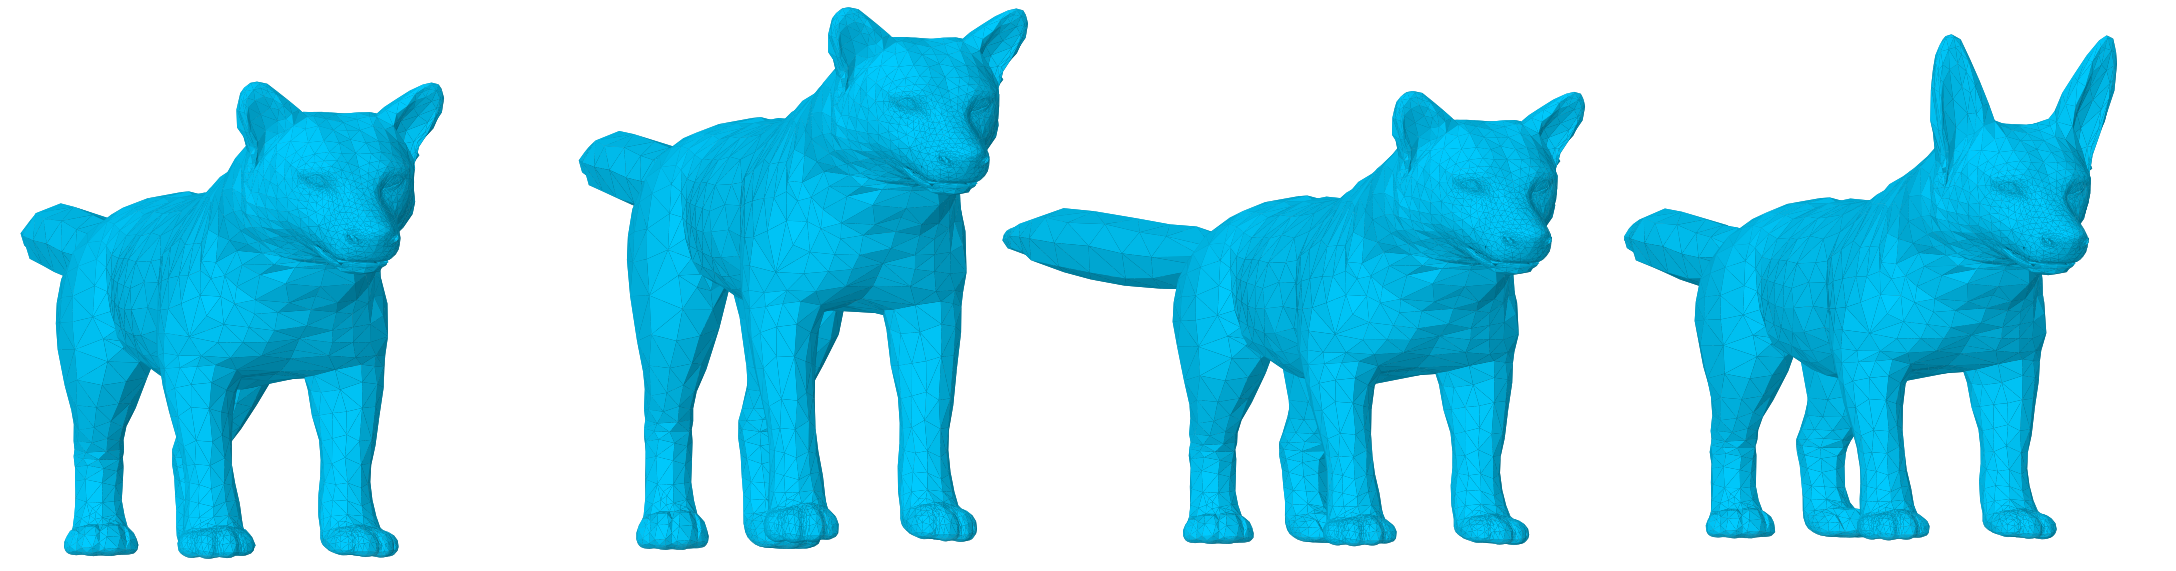
\includegraphics[width=.95\linewidth]{OllieFigs/all_shapevar.png}
    \caption{\textbf{Effect of varying SMBLD scale parameters}. 
    \emph{From left to right}: 
    Mean SMBLD model, 
    25\% leg elongation,
    50\% tail elongation,
    50\% ear elongation.}
    \label{fig:shape_variation}
\end{figure*}

\subsection{Learning a multimodal shape/scale prior}

The SMBLD shape prior is initialized by fitting the model to a set of $13$ artist-designed 3D dog meshes, downloaded from the internet and are similar in style to the SMAL toys. While the collection does offer a few more examples of dogs than used in the original SMAL set, the models still lack realism and are very constrained when compared to the 120 different breeds represented in the later test set. An energy minimization process is used to align the SMBLD vertices to each scan, in order to obtain a set of shape $\shape$, pose $\pose$ and $\scale$ parameters. 

\subsubsection{Fitting SMBLD to 3D scans}

Recall that SMBLD's shape $\shape$ and $\pose$ parameters are exactly as defined in SMAL, meaning there is no need to relearn (or adapt) the blend shape data $\mathcal{P}, \mathcal{S}$ or joint selectors $\jointselect$. The scale $\scale$ parameters, however, are novel to SMBLD. The goal of this section is to learn a new 3D prior over both shape and scale parameters which will initialize the later prior refined during the WLDO training loop. 

Note that fitting SMBLD to 3D scans emits much simpler optimization in comparison to 2D images, since the complete 3D information of the target mesh is available. In addition, the target meshes are not particularly detailed and are already aligned in the canonical T-pose, so we avoid need for a complex alignment technique as discussed in \Cref{chap:cgas}. 

An energy minimization process is used to align the SMBLD mesh to the 3D scans, subject to smoothing regularizers. The following energy formulation is minimized

\begin{equation}
    \E{opt} = \E{chamfer} + \E{laplacian} + \E{edge} + \E{normal}
\end{equation}
where each of these terms has a scalar weight $\lambda$. Here, $\W{chamfer}=\W{edge}=1.0$, $\W{normal}=0.01$ and $\W{laplacian}=0.1$. Optimization is run using stochastic gradient descent (SGD) with learning rate $1.0e^{-4}$ for $1000$ iterations. Further details on the specific energy terms are now provided.

\ss{Chamfer energy.} A measure of the average distance between vertices of the SMBLD mesh $V=F_v(\pose, \shape)$, and the target mesh vertices $V'$, when $p$ vertices $v_{i}, v'_{j}$ are sampled from each mesh respectively:
\begin{equation}
        \E{chamfer}(V, V') = \frac{1}{p} \sum_{i=1}^p \min_j^p  \left | v_{i} - v'_{j} \right |
\end{equation}

\ss{Uniform laplacian energy.} A measure of the mesh smoothness.

\ss{Edge energy.} This energy is equal to the average edge length across the mesh, and is used to encourage uniform distribution of vertices.

\ss{Normal energy.} This energy promotes consistency between adjacent faces. It is a measure of the average normal consistency between adjacent faces. For two faces with normals $\mathbf{n_0}$ and $\mathbf{n_1}$, the normal consistency is $1 - \frac{\mathbf{n_0} \cdot \mathbf{n_1}}{\left|\mathbf{n_0}\right|\left|\mathbf{n_1}\right|}$.

At the end of this process, we have a collection of fits $\left|(\pose,\shape)\right|_{\{i=1,...13\}}$ from which we can learn our unimodal pose and shape priors. As discussed, we evenutally use this unimodal shape prior to initialize our mixture shape prior, which is tuned with the expectation-maximization step in the training loop.

\subsubsection{Learning a unimodal shape prior}

Recall that the SMAL body shapes are represented by the linear function in \Cref{eqt:shapeblendshapes}. In this formulation, the matrix $S_{n}$ represents the orthonormal principal components of shape displacements. A consquence of the PCA construction is that the features in $\nshape$-dimensional parameter space (as they are linear combinations of the original features) are normally distributed with mean $\shapemu$ and covariance matrices $\shapecov$. With this construction, a likelihood function measures the probability of a given shape vector $\shape \in \R{\nshape}$

\begin{equation}
    \mathbb{P}_{\shape}(\shape) = (2\pi)^{-\frac{\nshape}{2}}\det(\shapecov)^{-\frac{1}{2}}e^{-\frac{1}{2}(\shape-\shapemu)^{T}\shapecov^{-1}(\shape-\shapemu)}
\end{equation}

For problems which aim to optimize $\shape$ as a free variable, the 3D shape prior is obtained by maximizing $\mathbb{P}_{\shape}(\shape)$ or equivalently, by minimizing the negative log likelihood

\begin{equation}
     -\ln\left[\mathbb{P}_{\shape}(\shape)\right] = -\frac{1}{2}\left[\ln\det(\shapecov) + \nshape\ln(2\pi) +  (\shape - \shapemu)^T\Sigma^{-1}(\shape-\shapemu)\right]
\end{equation}
Finally, terms with no dependency on $\shape$ can be dropped since they remain constant during the optimization. This reduces the formulation of the loss as the Mahalanobis distance of $\shapemu$

\begin{equation}
    \L{shape}(\shape;\shapemu,\shapecov) = (\shape - \shapemu)^{T}\shapecov^{-1}(\shape - \shapemu)
\end{equation}

A similar construction applies to the scale parameters $\scale$ with means and covariances computed from the 13 training scans. The scale loss function is therefore given as

\begin{equation}
    \L{scale}(\scale;\scalemu,\scalecov)= (\scale - \scalemu)^{T}\scalecov^{-1}(\scale - \scalemu)
\end{equation}

Continuing from here, it is convenient to group shape and scale parameters into a new shape-scale variable $\shapescale$ and the loss function can be grouped as follows
\begin{equation}
    \L{shape-scale}(\shapescale=\left[\shape,\scale\right];\shapescalemu=\left[\shapemu,\scalemu\right],\shapescalecov=\left[\shapecov,\scalecov\right]) = \L{shape}(\shape;\shapemu,\shapecov) + \L{scale}(\scale;\scalemu,\scalecov)
\end{equation}

% END PRELIMINARIES

% We have already seeen this formulation in Chapter 4.

% \subsubsection{Learning an improved prior via 3D model fitting}

% Recall that SMBLD is adapted from the SMAL~\cite{zuffi2017menagerie} deformable animal mesh, by including limb scaling parameters. A new shape prior is learnt by fitting this new SMBLD model, which comprises parameters for pose $\pose$ and shape $\beta$ (the latter of which now includes scaling parameters $\kappa$).

\subsubsection{Extending the formulation with a multimodal shape prior}

\def\imgweight{w}

The previous section introduced a unimodal, multivariate Gaussian prior, based on mean $\shapescalemu$ and covariance matrix $\shapescalecov$. However, enforcing this throughout training tends to result in predictions which appear similar in 3D shape, even when tested on dog images of different breeds. Diversity is improved among predicted 3D dog shapes by extending the above formulation to a Mixture of $M$ Gaussians prior.

Here, $\shapescalemu^{m}$, $\shapescalecov^{m}$ and $\shapescalepi^{m}$ are the mean, covariance and mixture weight respectively for Gaussian component 
$m$. For each component the mean is sampled from the existing unimodal prior and the covariance is set equal to the unimodal prior i.e. $\shapescalecov^{m} := \shapescalecov$. All mixture weights are initially set to $\frac{1}{M}$.

Each training image $i$ is assigned a set of latent variables $\{\imgweight_{i}^{1}, \dots, \imgweight_{i}^{M}\}$ encoding the probability of the dog shape in image~$i$ being generated by component~$m$. 

The mixture shape loss is given as:
\begin{align}
    \L{mixture}(\shapescale_{i}; \shapescalemu, \shapescalecov, \shapescalepi)
    =&
    \sum_{m=1}^M \shapepi^{m} \left[\L{shape-scale}(\shapescale_{i}; \shapescalemu^{m}, \shapescalecov^{m})\right]
\end{align}



% \section{Learning mixture shape prior.}
% This section contains additional detail for how we learn our mixture shape prior, using expectation maximization in-the-loop.


% Way more here, and include exampels